%%%%%%%%%%%%%%%%%%%%%%%%%%%%%%%%%%%%%%%%%
% Short Sectioned Assignment LaTeX Template Version 1.0 (5/5/12)
% This template has been downloaded from: http://www.LaTeXTemplates.com
% Original author:  Frits Wenneker (http://www.howtotex.com)
% License: CC BY-NC-SA 3.0 (http://creativecommons.org/licenses/by-nc-sa/3.0/)
%%%%%%%%%%%%%%%%%%%%%%%%%%%%%%%%%%%%%%%%%

%----------------------------------------------------------------------------------------
%	PACKAGES AND OTHER DOCUMENT CONFIGURATIONS
%----------------------------------------------------------------------------------------

\documentclass[paper=a4, fontsize=11pt]{scrartcl} % A4 paper and 11pt font size

% ---- Entrada y salida de texto -----

\usepackage[T1]{fontenc} % Use 8-bit encoding that has 256 glyphs
\usepackage[utf8]{inputenc}
%\usepackage{fourier} % Use the Adobe Utopia font for the document - comment this line to return to the LaTeX default

% ---- Idioma --------

\usepackage[spanish, es-tabla]{babel} % Selecciona el español para palabras introducidas automáticamente, p.ej. "septiembre" en la fecha y especifica que se use la palabra Tabla en vez de Cuadro

% ---- Otros paquetes ----

\usepackage{url} % ,href} %para incluir URLs e hipervínculos dentro del texto (aunque hay que instalar href)
\usepackage{amsmath,amsfonts,amsthm} % Math packages
%\usepackage{graphics,graphicx, floatrow} %para incluir imágenes y notas en las imágenes
\usepackage{graphics,graphicx, float} %para incluir imágenes y colocarlas

\usepackage{listings}	%para incluir remarcado para comandos bash

% Para hacer tablas comlejas
%\usepackage{multirow}
%\usepackage{threeparttable}

%\usepackage{sectsty} % Allows customizing section commands
%\allsectionsfont{\centering \normalfont\scshape} % Make all sections centered, the default font and small caps

\usepackage{fancyhdr} % Custom headers and footers
\pagestyle{fancyplain} % Makes all pages in the document conform to the custom headers and footers
\fancyhead{} % No page header - if you want one, create it in the same way as the footers below
\fancyfoot[L]{} % Empty left footer
\fancyfoot[C]{} % Empty center footer
\fancyfoot[R]{\thepage} % Page numbering for right footer
\renewcommand{\headrulewidth}{0pt} % Remove header underlines
\renewcommand{\footrulewidth}{0pt} % Remove footer underlines
\setlength{\headheight}{13.6pt} % Customize the height of the header

\numberwithin{equation}{section} % Number equations within sections (i.e. 1.1, 1.2, 2.1, 2.2 instead of 1, 2, 3, 4)
\numberwithin{figure}{section} % Number figures within sections (i.e. 1.1, 1.2, 2.1, 2.2 instead of 1, 2, 3, 4)
\numberwithin{table}{section} % Number tables within sections (i.e. 1.1, 1.2, 2.1, 2.2 instead of 1, 2, 3, 4)

\setlength\parindent{0pt} % Removes all indentation from paragraphs - comment this line for an assignment with lots of text

\newcommand{\horrule}[1]{\rule{\linewidth}{#1}} % Create horizontal rule command with 1 argument of height

\usepackage{booktabs}
\usepackage{tabularx}
\usepackage{multicol} 
\usepackage{hyperref}

%----------------------------------------------------------------------------------------
%	TÍTULO Y DATOS DEL ALUMNO
%----------------------------------------------------------------------------------------

\title{
\normalfont \normalsize 
\textsc{\textbf{Ingeniería del conocimiento (2020-2021)} \\ Máster en ingeniería informática \\ Universidad de Granada} \\ [25pt] % Your university, school and/or department name(s)
\horrule{0.5pt} \\[0.4cm] % Thin top horizontal rule
\huge Práctica 2: Desarrollo de un Sistema de Recomendación basado
en Filtrado Colaborativo \\ % The assignment title
\horrule{2pt} \\[0.5cm] % Thick bottom horizontal rule
}
\author{Manuel Orantes Taboada \\ \\ manuelorantes96@gmail.com \\ morantes96@correo.ugr.es \\ 77150692K} % Nombre y apellidos

\date{\normalsize\today} % Incluye la fecha actual

%----------------------------------------------------------------------------------------
% DOCUMENTO
%----------------------------------------------------------------------------------------

\begin{document}

\maketitle % Muestra el Título

\newpage %inserta un salto de página

\tableofcontents % para generar el índice de contenidos

\newpage

\section{Descripción}

La práctica consiste en hace un recomendados de películas a partir de la base de datos MovieLens. Es una base de datos que tiene 100000 valoraciones de 943 usuarios sobre 1682 películas. Se usarán estas valoraciones para crear un sistema que recomiende películas a un usuario siguiendo un sistema de vecino cercano. Para ello, se le pedirá al usuario que valore primero 20 películas aleatorias, según las cuales se pondrán recomendar películas después.

\section{Desarrollo de la práctica}
La práctica se ha realizado con el lenguaje python. Se han seguido las diapositivas del temario vistas en clase.

En primer lugar, hay una serie de líneas para parsear los archivos, y de este modo tener los datos en arrays y diccionarios de python.

Tenemos dos archivos .py. Veamos para que sirven ambos:

\subsection{CrearTablaSimilitud.py}
Este archivo será el encargado de:
\begin{itemize}
	\item Recoger los datos del usuario, preguntándole por 20 películas que deberá puntuar de 1 a 5.
	\item Crear la tabla de similitud, de todos los usuarios con el usuario que puntúa las 20 películas. 
\end{itemize}

Una vez que se han obtenido los resultados del usuario, se utiliza la similitud del coseno, vista en las transparencias de la clase. Por último, se exportan los datos en el fichero tablaSimilitud.txt, aunque realmente es un archivo .csv . Además, también se crea otro archivo, peliculasVisualizadas.txt (que también es un csv), en el que se guardarán los títulos de las películas vistas por el usuario (las 20 que se usaron al principio).

\subsection{recomendador.py}

En este archivo se leerán los datos, tanto proporcionados por MovieLens como los obtenidos en el paso anterior. Se usa la tabla de similitudes para calcular la puntuación de cada una de las películas, según las diapositivas del tema, y después se añaden, las que no haya visto el usuario. Por último, se ordenan según la puntuación.

\subsection{Extra}

Para finalizar, buscando información por Internet  encontré un programa que usa también el vecino cercano, pero que lo hace sobre las películas en sí. Busca las películas más similares a otra dada. Me pareció buena idea incorporar esta idea como extra, del modo que lo que hago es lo siguiente: En el paso anterior, me quedo con las 7 películas mejor valoradas. Después, completaré hasta 10 de la siguiente forma: de la película mejor valorada, cogeré las dos más similares a esta, siempre que no estén ya añadidas y no las haya visto el usuario. Cogeré también la más similar a la segunda película mejor valorada.

\section{Guía de usuario}
El uso es muy sencillo, solo hace falta tener los paquetes necesarios de python instalados (numpy , pandas, math, operator, scipy). Después, ejecutaremos CrearTablaSimilitud.py y responderemos a las preguntas introduciendo números del 1 al 5 (enteros y ambos incluidos). Este es el ejemplo de ejecución que yo he realizado:
\begin{figure}[H]
	\centering
	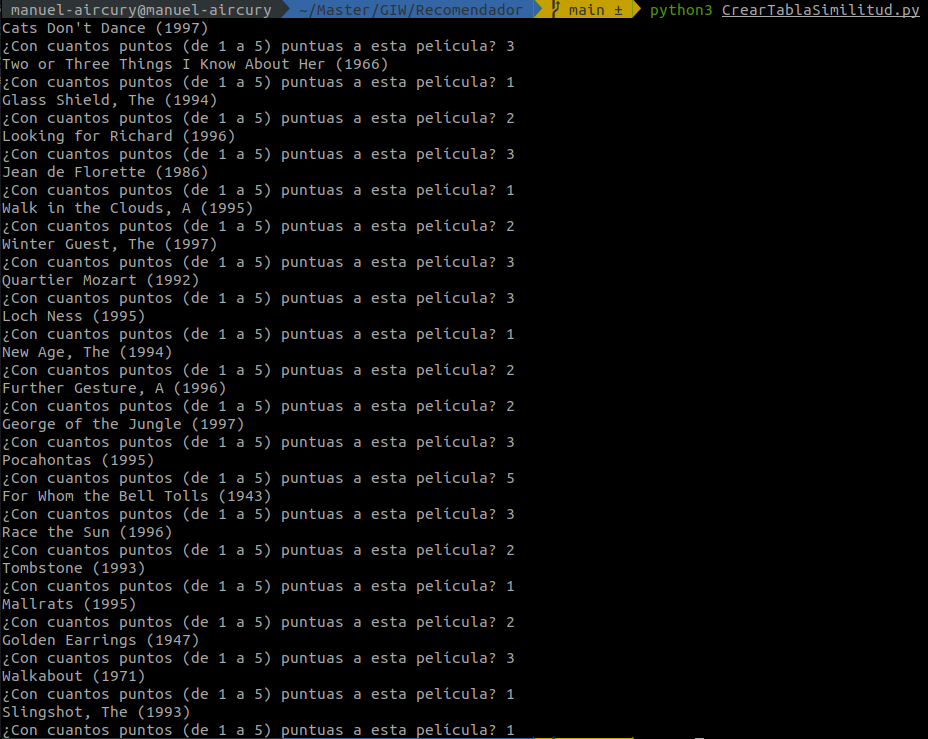
\includegraphics[width=0.7\linewidth]{Imagenes/screenshot001}
\end{figure}

Después, bastará con ejecutar recomendador.py, que devolverá una lista de las 10 películas recomendadas para tí.

\begin{figure}[H]
	\centering
	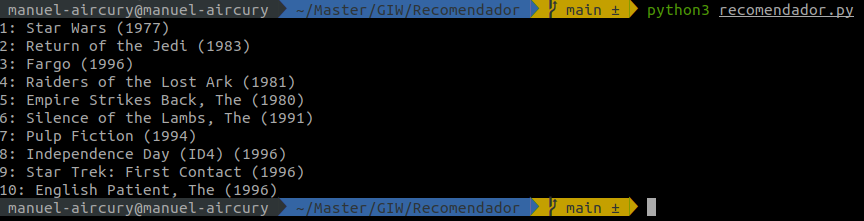
\includegraphics[width=0.7\linewidth]{Imagenes/screenshot003}
\end{figure}



\section{Bibliografía consultada}
Además de basarme en la propia práctica, he usado este tutorial:

\url{https://hendra-herviawan.github.io/Movie-Recommendation-based-on-KNN-K-Nearest-Neighbors.html}

\end{document}